\documentclass{article}

\usepackage[left=2cm,right=2cm,top=2cm,bottom=2cm]{geometry} 

\usepackage[utf8]{inputenc}   % otra alternativa para los caracteres acentuados y la "ñ"
\usepackage[           spanish % para poder usar el español
                      ,es-tabla % para los captions de las tablas
                       ]{babel}   
\decimalpoint %para usar el punto decimal en vez de coma para los números con decimales

%\usepackage{beton}
%\usepackage[T1]{fontenc}

\usepackage{parskip}
\usepackage{xcolor}

\usepackage{caption}

\usepackage{fancyvrb}

\usepackage{enumerate} % paquete para poder personalizar fácilmente la apariencia de las listas enumerativas

\usepackage{graphicx} % figuras
\usepackage{subfigure} % subfiguras

\usepackage{amsfonts}
\usepackage{amsmath}

\usepackage[formats]{listings}
\lstdefineformat{R}{~=\( \sim \)}
\lstset{basicstyle=\ttfamily,format=R}

\definecolor{gris}{RGB}{220,220,220}
	
\usepackage{float} % para controlar la situación de los entornos flotantes

\restylefloat{figure}
\restylefloat{table} 
\setlength{\parindent}{0mm}


\usepackage[bookmarks=true,
            bookmarksnumbered=false, % true means bookmarks in 
                                     % left window are numbered
            bookmarksopen=false,     % true means only level 1
                                     % are displayed.
            colorlinks=true,
            allcolors=blue,
            urlcolor=blue]{hyperref}
\definecolor{webblue}{rgb}{0, 0, 0.5}  % less intense blue


\title{\Huge SWAP: Clonar la información de un sitio web\vspace{10mm}}

\author{\huge David Cabezas Berrido \vspace{10mm} \\ 
  \huge dxabezas@correo.ugr.es \vspace{10mm}}

\begin{document}
\maketitle
\tableofcontents
\newpage

\section{Objetivos}

TODO

\section{Copiar archivos locales en equipos remotos: tar y scp}

Si queremos copiar el directorio \texttt{$\mathtt{\sim}$/directorio} de la máquina 1 a la 2, tenemos varias opciones.
Con el comando \textbf{tar}, realizamos en M1
\begin{lstlisting}
	tar czf - directorio | ssh dxabezas@192.168.56.102 'cat > ~/directorio.tgz'
\end{lstlisting}

El directorio es comprimido y con un cauce lo enviamos directamente al directorio \texttt{$\mathtt{\sim}$} de la máquina 2, sin ocupar
 espacio extra en la máquina 1.

\begin{itemize}
	\item La opción \texttt{c} (\texttt{create}) indica que queremos crear un nuevo archivo.
	\item La opción \texttt{z} (\texttt{gzip}) aplica la herramienta de compresión \texttt{gzip}.
	\item La opción \texttt{f} (\texttt{file}) indica el archivo a guardar.
\end{itemize}

Ahora en la máquina 2 comprobamos con \texttt{ls} que el archivo ha sido recibido el archivo \texttt{$\mathtt{\sim}$/directorio.tgz},
y procedemos a extraerlo con
\begin{lstlisting}
tar -xzf directorio.tgz -C ~/
\end{lstlisting}

\begin{itemize}
	\item La opción \texttt{x} (\texttt{extract}, \texttt{get}) indica que queremos extraer archivos.
	\item La opción \texttt{z} (\texttt{gzip}) aplica la descompresión de \texttt{gnupzip}.
	\item La opción \texttt{C} (\texttt{directory}) indica el directorio donde queremos extraer los archivos.
\end{itemize}

Opcionalmente, se puede usar la opción \texttt{v} (\texttt{verbose}) para que liste los archivos que va comprimiendo o extrayendo.

Señalamos también la opción \texttt{u} (\texttt{update}), que permite añadir al archivo \texttt{.tgz} sólo los archivos que han sido
 modificados desde la última copia. La desventaja es que no funciona en ficheros comprimidos.

\begin{figure}[H]
	\centering
	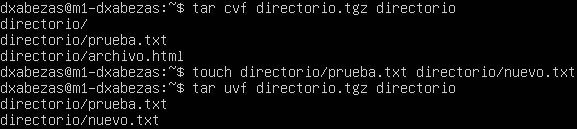
\includegraphics[width=140mm]{imgs/tar-update}
	\caption{Suprimiendo la opción \texttt{z} por incompatibilidad, guardamos el contenido del directorio en un fichero \texttt{.tgz}.
	Editamos un archivo existente y creamos uno nuevo, y utilizamos \texttt{update} en lugar de \texttt{create} para que añada sólo los
	archivos recientes.}
	\label{fig:tar-update}
\end{figure}

La otra alternativa es la herramienta \textbf{SCP} (Secure Copy), que usa SSH para hacer copias seguras de archivos.

\begin{figure}[H]
	\centering
	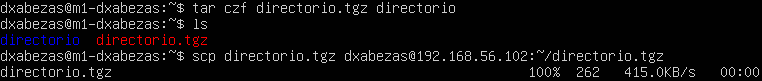
\includegraphics[width=160mm]{imgs/scp}
	\caption{En la máquina 1 comprimimos el directorio y después lo enviamos por SSH a la máquina 2 con SCP.}
	\label{fig:scp}
\end{figure}

Ya podemos extraer los archivos en la máquina 2 como hicimos antes.

Esta opción tiene la desventaja de que la copia ocupa espacio en M1, podemos evitarlo utilizando:

\begin{figure}[H]
	\centering
	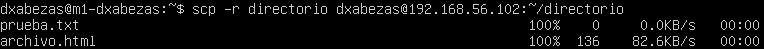
\includegraphics[width=160mm]{imgs/scp2}
	\caption{Eviamos el directorio directamente desde M1 a M2, sin comprimir.}
	\label{fig:scp2}
\end{figure}

\begin{itemize}
	\item La opción \texttt{r} indica que copie directorios enteros de forma recursiva.
\end{itemize}

Señalamos cuatro opciones de SCP que pueden sernos de utilidad:
\begin{itemize}
	\item La opción \texttt{o} permite pasar opciones a SSH en el formato del fichero de configuración del cliente
	 (\texttt{ssh\_config}).
	\item La opción \texttt{P} permite seleccionar el puerto de SSH, es útil cuando no es el 22 (default).
	\item La opción \texttt{q} desabilita los mensajes, útil si hay muchos archivos y no queremos que se nos llene la terminal.
	\item La opción \texttt{v}, como de costumbre, imprime mensajes sobre el progreso. Tanto de SCP como de SSH.
\end{itemize}

Notamos que en ningún momento nos pide la contraseña porque configuramos el acceso sin contraseña de SSH en la anterior práctica.

\section{Sincronizar archivos locales en equipos remotos: rsync}

Ejecutamos \texttt{sudo apt install rsync}, y descubrimos que ya está instalado en ambas máquinas.

Hacemos al usuario dueño del directorio \texttt{/var/www}:

\begin{verbatim}
	sudo chown dxabezas:dxabezas -R /var/www
\end{verbatim}

Desde la máquina 2, ejecutamos lo siguiente.

\begin{figure}[H]
	\centering
	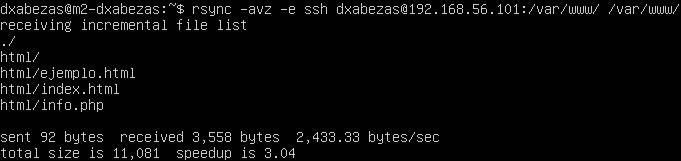
\includegraphics[width=150mm]{imgs/rsync}
	\caption{Desde M2, nos conectamos a M1 y sincronizamos los contenidos del directorio \texttt{/var/www}.}
	\label{fig:rsync}
\end{figure}

Ahora podemos conectarnos desde el navegador al servidor de Apache2 de M2, que sirve los contenidos que originalmente eran de 
M1.

\begin{figure}[H]
	\centering
	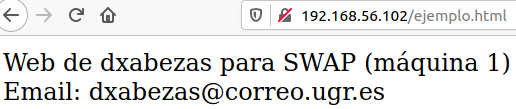
\includegraphics[width=130mm]{imgs/rsync-example}
	\caption{Ahora el directorio \texttt{/var/www} de M2 tiene los contenidos que originalmente eran de M1.}
	\label{fig:rsync-example}
\end{figure}

Explicamos el significado de las opciones:
\begin{itemize}
	\item La opción \texttt{a} (\texttt{archive}) indica que usamos recursividad (para copiar los directorios completos) y preservar la estructura de archivos.
	Una excepción son los enlaces duros, que deben explicitarse con la opción \texttt{H}.
	\item La opción \texttt{v} para verbose.
	\item La opción \texttt{z} para que los archivos se transfieran comprimidos.
	\item La opción \texttt{e} para especificar el shell remoto a utilizar, por defecto SSH.
\end{itemize}

Otras opciones que pueden ser útiles:
\begin{itemize}
	\item La opción \texttt{p} para preservar los permisos, implícito en \texttt{a}.
	\item La opción \texttt{r} para recursividad en los directorios.
	\item La opción \texttt{t} para preservar los tiempos de modificación originales, también implícito en \texttt{a}.
\end{itemize}

La \texttt{--delete} indica que se borren de M2 los archivos que se hayan eliminado en M1, de tal forma que la copia sea idéntica.
Por último, la opción \texttt{--exclude} se usa para no copiar ciertos archivos, por ejemplo: \texttt{--exclude=**/patata.txt} no copiará
el fichero \texttt{/var/www/patata.txt} de M1 a M2.

Igualmente, tampoco se nos ha solicitado la contraseña del usuario por la configuración de SSH que realizamos en la anterior práctica.

\section{Acceso sin contraseña con SSH}

En la anterior práctica configuramos el acceso sin contraseña por SSH con la utilidad \texttt{ssh-copy-id}. Hablaremos de algunas opciones
para esta tarea y explicaremos la alternativa manual.

Cuando se genera la clave con \texttt{ssh-keygen}, la opción \texttt{-t} se utiliza para indicar el tipo de clave: rsa, dsa (digital
 signature algorithm, para firma digital), ecdsa (elliptic curve DSA). La opción \texttt{-f} se utiliza para indicar el fichero con la clave,
 si la omitimos lo preguntará luego. Por defecto el fichero con la clave privada es \texttt{$\mathtt{\sim}$/.ssh/id\_rsa}, y para la clave
 pública se añade la extensión \texttt{.pub}. También la opción \texttt{-b} permite especificar la longitud (en bits) de la clave, por
 defecto 2048.
 
 En caso de no utilizar una clave en el archivo por defecto, debemos indicar con la opción \texttt{-i} la ruta de la clave tanto para la
 copia de la clave pública:
 \begin{verbatim}
 	ssh-copy-id -i /ruta/clave.pub usuario@ip
 \end{verbatim}
 como para la privada al acceder:
\begin{verbatim}
		ssh -i /ruta/clave usuario@ip
\end{verbatim}

Por último, podemos visualizar la fingerprint y el randomart de la clave con la siguiente orden:

\begin{figure}[H]
	\centering
	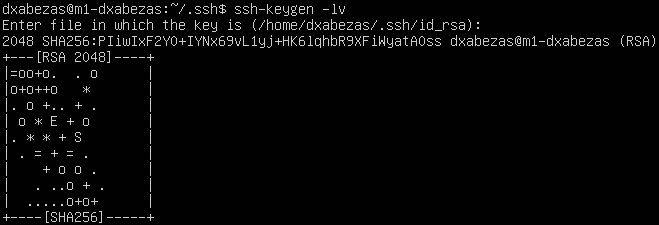
\includegraphics[width=120mm]{imgs/ssh-fingerprint}
	\caption{La opción \texttt{-l} permite visualizar la fingerprint de una clave existente, y añadir \texttt{-v} permite visualizar
		su randomart.}
	\label{fig:ssh-fingerprint}
\end{figure}

Finalmente, configuraremos el acceso sin contraseña manualmente. Para ello, deshaceremos primero la configuración automática de la práctica 1, lo que
ya dará una pista de como se hace la configuración manual. Las claves públicas guardadas están en el fichero \texttt{$\mathtt{\sim}$/.ssh/authorized\_keys}
del servidor (M1), ahí encontramos la que guardamos con \texttt{ssh-copy-id}.

\begin{figure}[H]
	\centering
	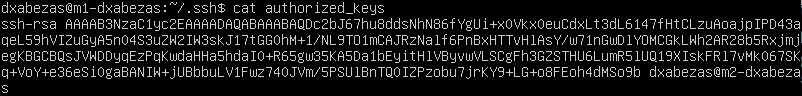
\includegraphics[width=140mm]{imgs/authorized-keys}
	\caption{La clave pública de M2 guardada en M1. Se puede ver que es de M2 en el final de la clave, porque lo que indicamos con la opción
		 \texttt{-C} al crear la clave.}
	\label{fig:authorized-keys}
\end{figure}

Borramos la clave con nano, y comprobamos que efectivamente nos pide la contraseña para acceder.

Ahora escribimos de forma manual la clave que generamos en la primera práctica de M2 en el fichero \texttt{authorized\_keys} de M1.

\begin{figure}[H]
	\centering
	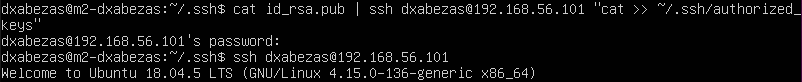
\includegraphics[width=140mm]{imgs/ssh-manual}
	\caption{Copiamos manualmente la clave pública de M2 en M1, y ya podemos acceder sin contraseña.}
	\label{fig:ssh-manual}
\end{figure}

\section{Programación de tareas: crontab}

En la máquina 2, utilizamos el demonio cron para que sincronice su directorio \texttt{/var/www} con el de M1 cada hora,
concretamente en el minuto 0. Esto lo conseguimos haciendo \texttt{crontab -e} en la máquina 2 y añadiendo la siguiente línea:
\begin{verbatim}
	# m h dom mon dow command
	0 * * * * rsync -avz -e ssh dxabezas@192.168.56.101:/var/www/ /var/www/ --delete
\end{verbatim}
Como se nos indica el fichero, no hace falta escribir el usuario porque ya sabe cuál es. Esperamos un poco y comprobamos que se sincroniza
 correctamente.

Hemos usado \texttt{--delete} para que el contenido de las carpetas sea idéntico.

Ahora señalaremos algunas opciones avanzadas para crontab. En primer lugar, el carácter \texttt{-} puede usarse para indicar intervalos, y
el carácter \texttt{/} para indicar saltos. Por ejemplo, si ponemos \texttt{0 12 1-15/3 * *}, la tarea se ejecutará los días 1,4,7,10,12 y 15
de cada mes a las 12 del mediodía.

También tenemos atajos, que se marcan con el carácter \texttt{@}. Por ejemplo, \texttt{@weekly} equivale a \texttt{0 0 * * 0}, que ejecuta
la tarea cada domingo (día 0) a las 00:00. De igual forma, existen \texttt{@yearly} y \texttt{@annually} para ejecutar la tarea el 1 de
enero a las 00:00; y \texttt{@hourly}, \texttt{@daily} y \texttt{@monthly}.

Finalmente tenemos \texttt{@reboot}, que lanza la tarea tras cada vez que apagamos y encendemos la máquina.

\end{document}
